\documentclass[12pt]{report}
\usepackage[francais]{babel}
\usepackage{ucs}
\usepackage[utf8x]{inputenc}
\usepackage{amsmath}
\usepackage{graphicx}
\usepackage{hyperref}
%\usepackage[latin1]{inputenc}
\usepackage[T1]{fontenc}

\title{%
    \begin{minipage}\linewidth
        \centering
        Rapport projet 1A
        \vskip3pt
        \large structures de donnée, algorithmique
        \vskip5pt
        \large \url{https://github.com/BCourteaud76/projet1A}
    \end{minipage}
}

%\title{Rapport projet 1A Structures de données algorithmique}
%\subtitle{Structures de données algorithmique}

\author{Paul Margerie \& Timothée Kocev}
\date{28 Mai 2019}

\begin{document}

\maketitle
%\makesubtitle
\renewcommand{\contentsname}{Sommaire} % Dans le corps du document,avant la commande \tableofcontents.
\renewcommand{\chaptername}{Chapitre} % Dans le corps du document,avant la commande \tableofcontents.
\tableofcontents

\chapter{Implantation}

%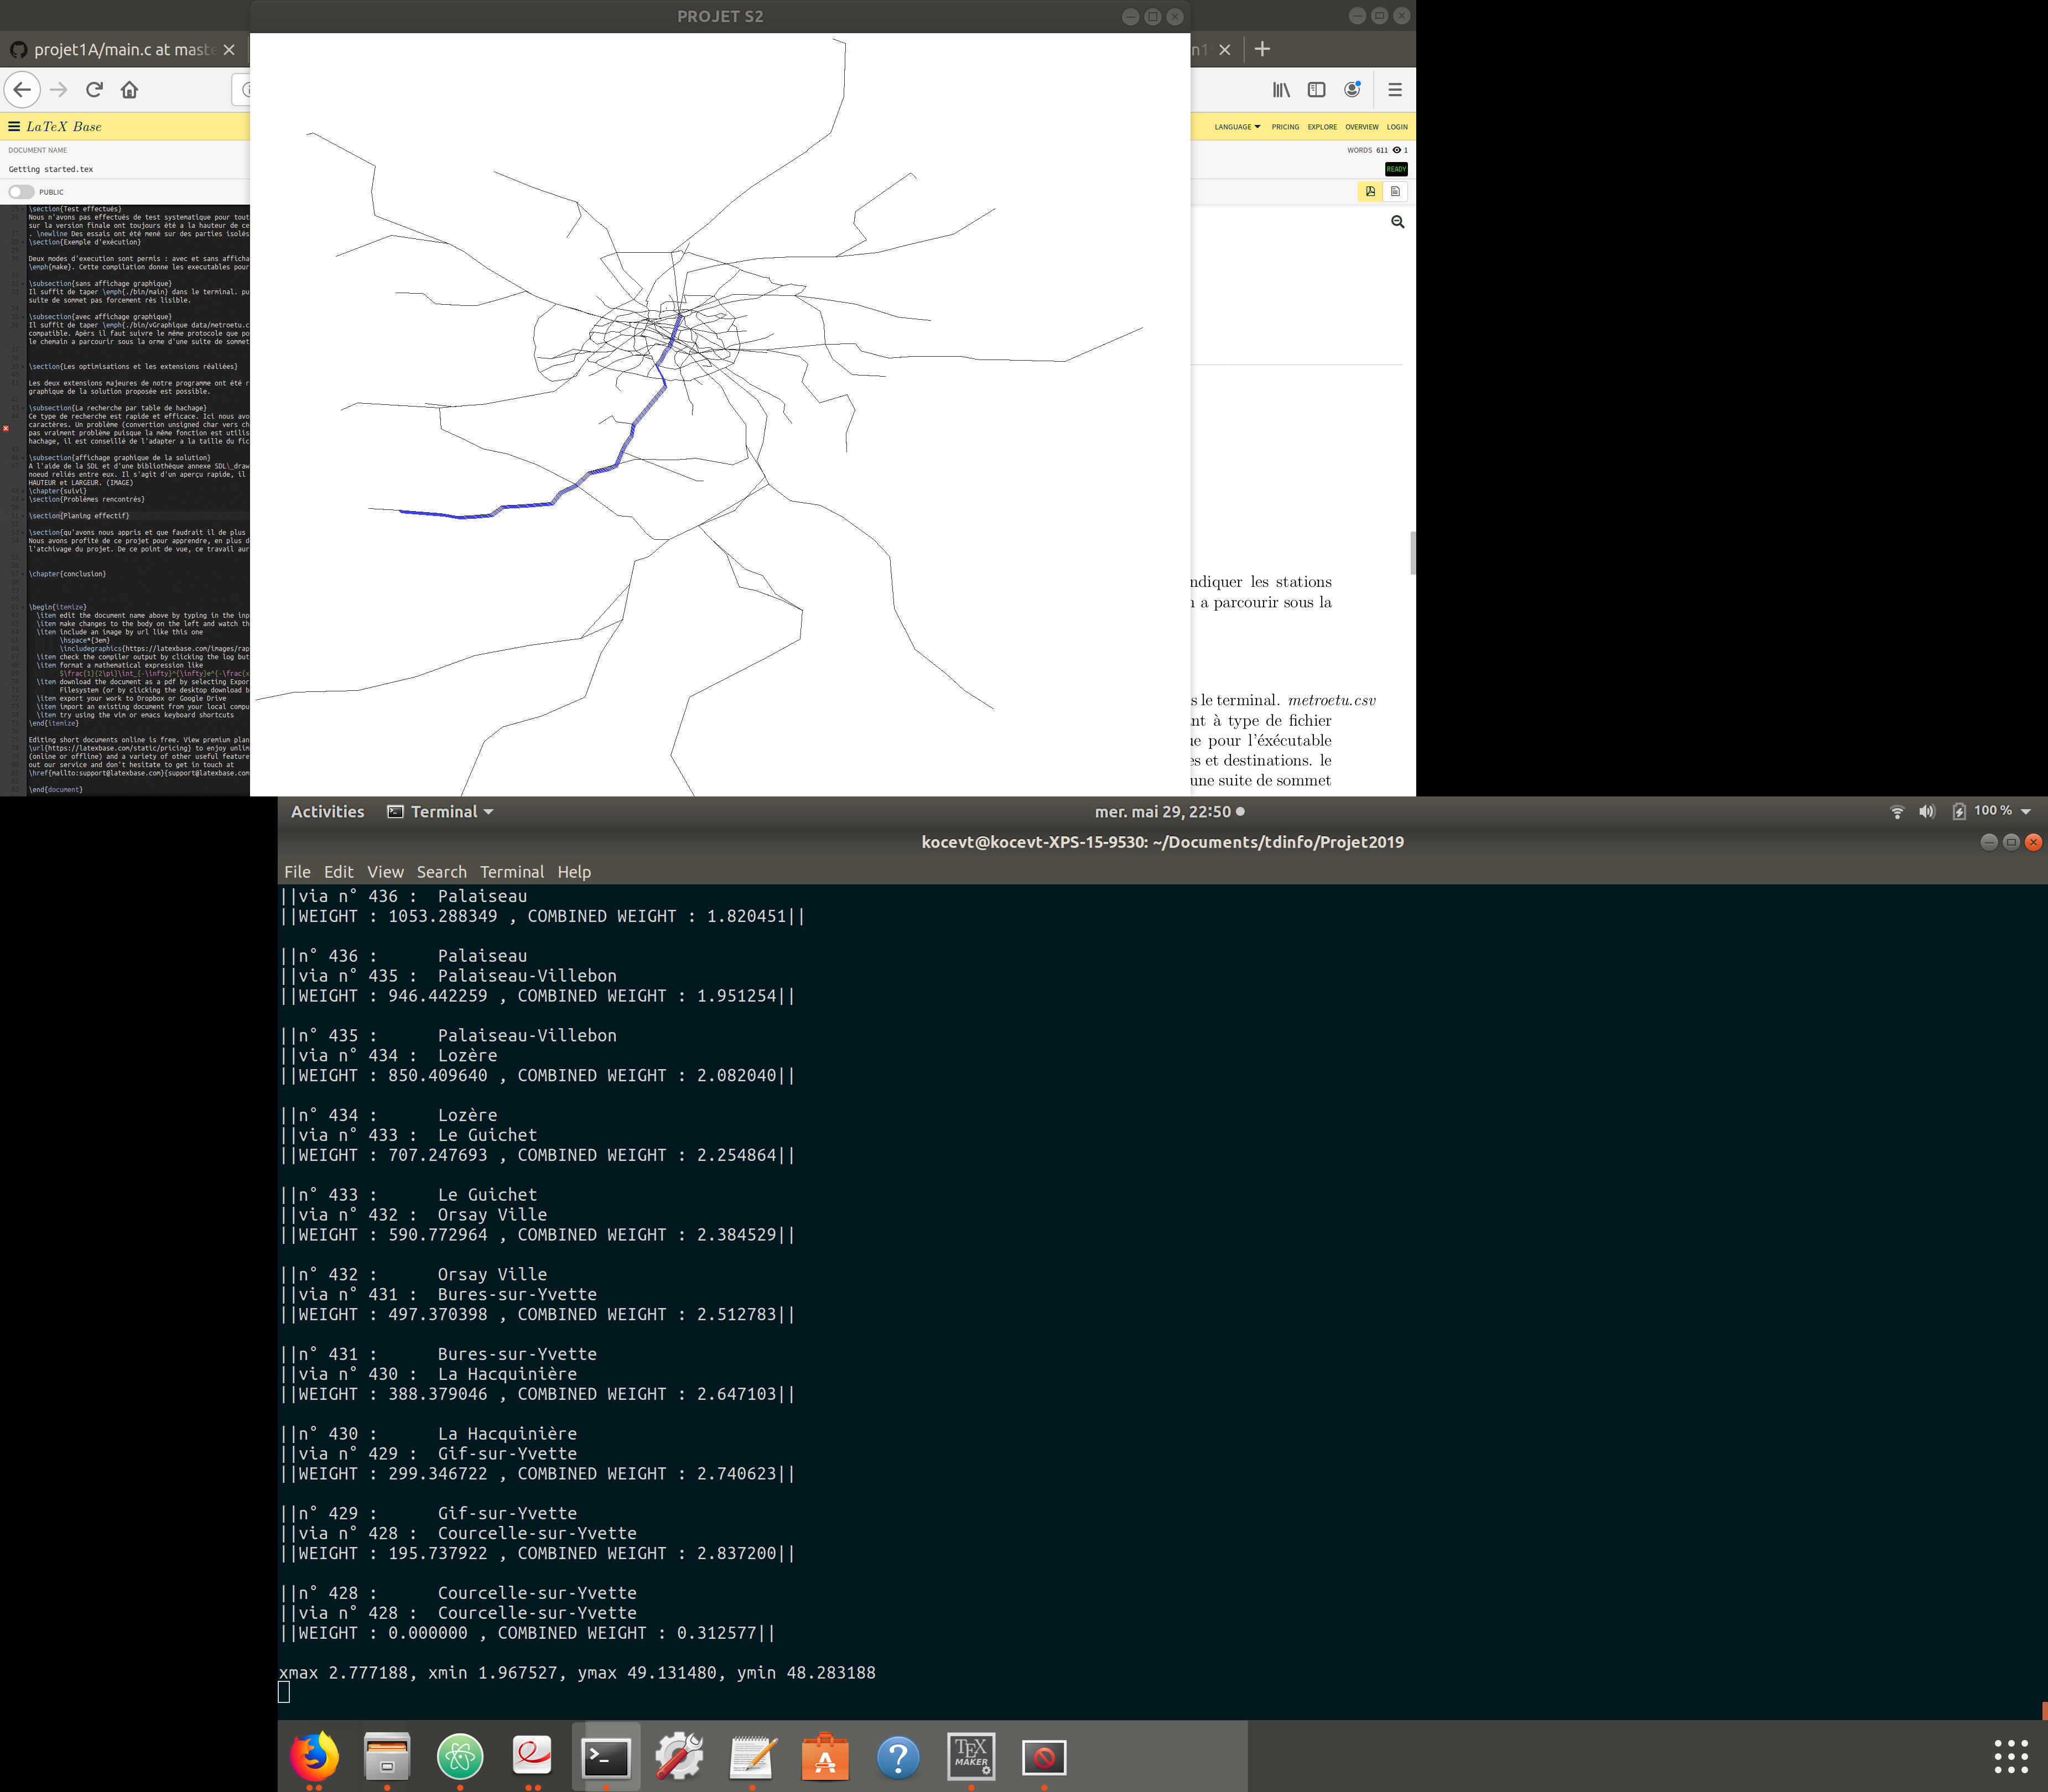
\includegraphics{images/essai.png}

\section{État du logiciel ; ce qui fonctionne, ce qui ne fonctionne pas}
Le logiciel fonctionne comme il doit sur les différents essais que nous avons mené. Un bug est toujours possibles pour certaines sommets. \newline Nous avons un problème de libération mémoire. certaines allocations ne sont pas libérées à la fin, mais nous n'arrivons pas à cerner d'où vient le problème.

\section{Test effectués}
Nous n'avons pas effectués de test systématiques pour toutes les combinaisons de sommet, mais des séries de tests ont été effectuées avec différentes stations. Les résultats sur la version finale ont toujours été a la hauteur de ce que nous espérions. L'itinéraire semble parfois pas tout à fait optimal mais le résultat a toujours été cohérent
. \newline Des essais ont été mené sur des parties isolés du programme lors de le conception des différentes parties.
\section{Exemple d'exécution}

Deux modes d'exécution sont permis : avec et sans affichage graphique. dans les deux cas, il faut se placer dans le répertoire du logiciel et compiler avec la commande \emph{make}. Cette compilation donne les exécutables pour les deux mode.


\subsection{sans affichage graphique}
Il suffit de taper \emph{./bin/main} dans le terminal. puis indiquer les stations origines et destinations. le programme affiche le chemin a parcourir sous la orme d'une suite de sommet pas forcement très lisible.

\subsection{avec affichage graphique}
Il suffit de taper \emph{./bin/vGraphique data/metroetu.csv} dans le terminal. \emph{metroetu.csv} peut être remplacer par m'importe quel chemin menant à type de fichier compatible. Après il faut suivre le même protocole que pour l'exécutable sans affichage graphique puis indiquer les stations origines et destinations. le programme affiche le chemin a parcourir sous la orme d'une suite de sommet pas forcement très lisible.


\section{Les optimisations et les extensions réalisées}

Les deux extensions majeures de notre programme ont été réalisées : il est possible de faire la recherche de la station grâce à une table de hachage et un affichage graphique de la solution proposée est possible.

\subsection{La recherche par table de hachage}
Ce type de recherche est rapide et efficace. Ici nous avons fait le choix d'une fonction de hachage particulièrement simple qui ne fait que la somme des valeurs ASCII des caractères. Un problème (conversions unsigned char vers char ?) donnait parfois un hach négatif. Ce problème à été résolu par l'ajout d'une valeur absolue. Chose qui ne pose pas vraiment problème puisque la même fonction est utilisée pour le remplissage et la recherche. Une macro, TAILLE\_TAB\_HACH, permet de définir la taille de la table de hachage, il est conseillé de l'adapter a la taille du fichier lu (mis à 400 pour le fichier metroetu d'environ 750 lignes).

\subsection{affichage graphique de la solution}
A l'aide de la SDL et d'une bibliothèque annexe SDL\_draw on réalise l'affichage des réseaux contenu dans les fichiers. Pour se faire on trace des lignes droite entre chaque noeud reliés entre eux. Il s'agit d'un aperçu rapide, il est possible de modifier l'échelle d'affichage dans graphic.h en modifiant les macros/variables pre-processeur HAUTEUR et LARGEUR. (IMAGE)
\chapter{suivi}
\section{Problèmes rencontrés}

Nous avons rencontrés pas mal de petits problèmes au cours de la réalisation de ce projet, la plus part du temps du a notre faute et au fait que nous avons encore beaucoup à apprendre pour avoir un code efficace. Une difficulté supplémentaire c'est tout de même ajoutée lors de la table de hachage. il y avait pas mal de caractères indésirables sur les lignes des noms des station. Il a aussi fallu trouver une solution pour récupérer une chaîne de caractères avec des espaces. Une première tentative avec \emph{gets} marchait, mais pas sur tous les ordinateurs (fonction dépréciée a partir du C99) on a donc réutiliser \emph{scanf} avec une option pour accepter tous les caractères sauf le retour chariot. Une autre fonction a du être ajouter pour nettoyer un peu le stdin avant la saisie suivante.

\section{Planning effectif}

Nous avons plutôt réussit à bien gérer notre temps, malgré une première séance consacrée a une prise en main un peu longue de GitHub. A chaque fin de séance, ou encours de séance si le débug n'a pas été trop long, les objectif sont fixés pour la semaine suivante. \newline La première séance à aussi permis de structurer nos fichiers avec l'arborescence séparant les différents types de fichiers.

\section{qu'avons nous appris et que  plus ?}
Nous avons profité de ce projet pour apprendre, en plus de la gestion des structures de donnée, a utiliser LaTeX pour la rédaction de ce rapport et GitHub pour le partage et l'archivage du projet. De ce point de vue, ce travail aura été d'autant plus instructif et enrichissant.


\chapter{conclusion}

Ce projet nous a pris beaucoup de temps, surtout avec les petites contraintes que nous nous sommes fixées, mais il a été très instructif. De plus ce projet est assez motivant car le logiciel est quand même très proche du quotidien. 

\end{document}